\documentclass[a4paper,11pt]{article}

% Kodovani (cestiny) v dokumentu: utf-8
%\usepackage[cp1250]{inputenc}	% Omezena stredoevropska kodova stranka, pouze MSW.
\usepackage[utf8]{inputenc}	% Doporucujeme pouzivat UTF-8 (unicode).

\usepackage[margin=2cm]{geometry}
\newtoks\jmenopraktika \newtoks\jmeno \newtoks\datum
\newtoks\obor \newtoks\skupina \newtoks\rocnik \newtoks\semestr
\newtoks\cisloulohy \newtoks\jmenoulohy
\newtoks\tlak \newtoks\teplota \newtoks\vlhkost

\jmenopraktika={Fyzikální praktikum 1}
\jmeno={Lukáš Lejdar}
\datum={15. října 2024}
\obor={F}
\skupina={Út 16:00}

\cisloulohy={8}
\jmenoulohy={Měření parametrů zobrazovacích soustav}

\tlak={101{,}35}
\teplota={21,1}
\vlhkost={47,7}


%%%%%%%%%%% Uzitecne balicky:
\usepackage[czech]{babel}
\usepackage{graphicx}

\usepackage{graphicx}
\usepackage{amsmath}
\usepackage{xspace}
\usepackage{url}
\usepackage{indentfirst}
\usepackage{wrapfig}
\usepackage{xcolor}
\usepackage{subfig}
\usepackage{subcaption}
\usepackage{enumitem}
\usepackage{tikzsymbols}
\usepackage{mathtools}
\usepackage{newfloat}
\usepackage{multirow}


%%%%%% Zamezeni parchantu:
\widowpenalty 10000 \clubpenalty 10000 \displaywidowpenalty 10000
%%%%%% Parametry pro moznost vsazeni vetsiho poctu obrazku na stranku
\setcounter{topnumber}{3}	  % max. pocet floatu nahore (specifikace t)
\setcounter{bottomnumber}{3}	  % max. pocet floatu dole (specifikace b)
\setcounter{totalnumber}{6}	  % max. pocet floatu na strance celkem
\renewcommand\topfraction{0.9}	  % max podil stranky pro floaty nahore
\renewcommand\bottomfraction{0.9} % max podil stranky pro floaty dole
\renewcommand\textfraction{0.1}	  % min podil stranky, ktery musi obsahovat text
\intextsep=8mm \textfloatsep=8mm  %\intextsep pro ulozeni [h] floatu a \textfloatsep pro [b] or [t]

% Tecky za cisly sekci:
\renewcommand{\thesection}{\arabic{section}.}
\renewcommand{\thesubsection}{\thesection\arabic{subsection}.}
% Jednopismenna mezera mezi cislem a nazvem kapitoly:
\makeatletter \def\@seccntformat#1{\csname the#1\endcsname\hspace{1ex}} \makeatother
%
\newcommand{\vsn}[4]{\ensuremath{#1 =} #2(#3)\,#4}
\newcommand{\vrn}[6]{\ensuremath{#1 =} (#2 $\pm$ #3)\,#4 ($p=$ #5\,\%, $\nu=$ #6)}

\newcommand*\circled[1]{\tikz[baseline=(char.base)]{
		\node[shape=circle,draw,inner sep=1pt] (char) {#1};}}

%%%%%%%%%%%%%%%%%%%%%%%%%%%%%%%%%%%%%%%%%%%%%%%%%%%%%%%%%%%%%%%%%%%%%%%%%%%%%%%
% Zacatek dokumentu
%%%%%%%%%%%%%%%%%%%%%%%%%%%%%%%%%%%%%%%%%%%%%%%%%%%%%%%%%%%%%%%%%%%%%%%%%%%%%%%

\begin{document}

\thispagestyle{empty}

{
\begin{center}
\sf 
{\Large Ústav fyziky a technologií plazmatu Přírodovědecké fakulty Masarykovy univerzity} \\
\bigskip
{\huge \bfseries FYZIKÁLNÍ PRAKTIKUM} \\
\bigskip
{\Large \the\jmenopraktika}
\end{center}

\bigskip

\sf
\noindent
\setlength{\arrayrulewidth}{1pt}
\begin{tabular*}{\textwidth}{@{\extracolsep{\fill}} l l}
\large {\bfseries Zpracoval:}  \the\jmeno & \large  {\bfseries Naměřeno:} \the\datum\\[2mm]
\large  {\bfseries Obor:} \the\obor  \hspace{40mm}  {\bfseries Skupina:} \the\skupina %
&\large {\bfseries Testováno:}\\
\\
\hline
\end{tabular*}
}

\bigskip

{
\sf
\noindent \begin{tabular}{p{4cm} p{0.6\textwidth}}
\Large  Úloha č. {\bfseries \the\cisloulohy:} \par
\smallskip
$T=\the\teplota$~$^\circ$C \par
$p=\the\tlak$~kPa \par
$\varphi=\the\vlhkost$~\%
&\Large \bfseries \the\jmenoulohy  \\[2mm]
\end{tabular}
}

\vskip1cm

\section{Úvod}

\section{Postup měření}

\subsection{Měření ohniskové vzdálenosti}

Budu používat zápornou znaménkovou konvenci na straně předmětu od čočky a kladnou čárkovanou na straně obrazu. Proměná $ a $ obecně označuje některou vzdálenost objektu od čočky, $ f $ ohniskovou vzdálenost a $ \beta = \frac{y'}{y} = \frac{a'}{a} $ příčné zvětšení. Ze zobrazovací rovnice se nabízí několik způsobů měření ohniskové vzdálenosti spojky.

\begin{enumerate}[label=\bfseries\tiny\protect\circled{\small\arabic*}]
    \item \textbf{Přímá metoda : }  Měří se vzdálenosti obrazu a předmětu a platí
        \begin{equation}
        f' = \frac{aa'}{a - a'}
        \end{equation}

    \item \textbf{Pomocí příčného zvětšení : } Měří se příčné zvětšení $ \beta $ a některá ze vzdáleností od čočky

        \begin{equation}
        f' = \frac{a'}{1 - \beta} = \frac{a \beta}{ 1 - \beta}
        \end{equation}

    \item \textbf{Besselova metoda : } Pro každou vzdálenost předmětu od stínítka $ d = |a| + |a'| > 4f$ , existují 2 polohy čočky takové, že předmět je na stínítku ostrý. Phybuju čočkou namísto stínítka a hledám tyto 2 polohy. Jejich vzdálenost označím $ \Delta = |a_1'| - |a_2'| = |a_2| - |a_1|$ a ohniskovou vzdálenost potom spočítám podle

        \begin{equation}
        f' = \frac{d^2 - \Delta^2}{4d}
        \end{equation}
\end{enumerate}

V případě rozptylky je potřeba zobrazovat neskutečný předmět, aby šlo pozorovat skutečný obraz. Takový předmět zajistím spojkou, která bude mezi předmětem a rozptylkou. Znám-li polohu rozptylky $ R $, polohu obrazu spojky $ A > R $ a polohu obrazu rozptylky A', můžu do vztahu (1) dosadit

\begin{equation}
a = A - R \quad \quad  a' = A' - R
\end{equation}

\subsection{Měření křivosti kulové čočky}

Poloměr křivosti $ r $ kulové čočky, budu měřit sférometrem. Je to zařízení s  kruhovým výřezem o poloměru $ z $ a posuvným čidlem uprostřed, které dokáže s velkou přesností určit rozdíl výšek. Jeho přiložením na čočku vytnu kulovou výseč o výšce $ h $ a základně $ z $, ze kterých dopočítám $ r $ podle

\begin{equation}
r = \frac{h^2 + z^2}{2h}
\end{equation}

\begin{figure}[htpb]
    \begin{minipage}[b]{.45\linewidth}
        \centering
        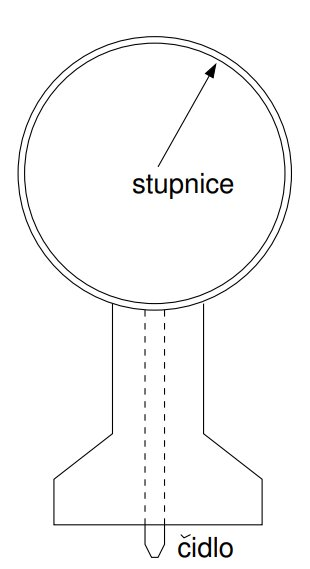
\includegraphics[width=0.4\textwidth]{sferometr.jpg}
        \caption{Sférometr}
    \end{minipage} 
    \begin{minipage}[b]{.5\linewidth}
        \centering
        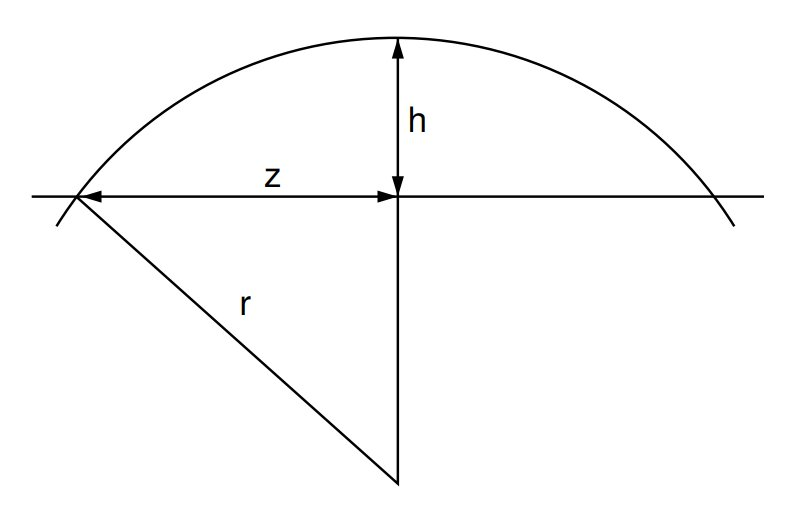
\includegraphics[width=0.9\textwidth]{kulova_plocha.jpg}
        \caption{Určení poloměru křivosti kulové plochy}
    \end{minipage} 
\end{figure}

Z poloměrů křivosti obou stran a ohniskové vzdálenosti se v případě tenkých čoček dá vyjádřit index lomu materiálu ze vztahu 

\begin{equation}
\frac{1}{f'} = (n - 1)(\frac{1}{r_1} - \frac{1}{r_2})
\end{equation}

\newpage
\section{Výsledky měření}

\subsection{Stanovení ohniskové vzdálenosti tenké spojky}

Na optickou lavici jsem za sebe postavil zdroj světla, spojku a stínítko. Našel jsem několik konfigurací této soustavy, kdy se obraz na stínítku jevil ostrý a pro každou odečetl vzdálenost a velikost předmětu i obrazu. Změřené hodnoty jsou uvedené v tabulce 1 spolu s výslednou ohniskovou vzdáleností $ f_p' $ podle vztahu (1), a $ f_{\beta 1}' = f(\beta, a) $ a $ f_{\beta 2}' = f(\beta, a') $ podle vztahu (2). Zprůměrováním hodnot jsem dostal

\begin{align*}
f_{\beta 1}' = 0.160 \pm 0.001 \text{ m} \\
f_{\beta 2}' = 0.169 \pm 0.009 \text{ m} \\
f_p' =  0.165 \pm 0.005 \text{ m}
\end{align*}


\begin{table}[htpb]
    \centering
    \begin{tabular}{cccc | ccc}
        $ a $ (m) & $ a' $ (m) & $ y $ (m) & $ y' $ (m) & $ f_p' $ (m) & $ f_{\beta 1}' $ (m) & $ f_{\beta 2}' $ (m)  \\ \hline
        -0.260 & 0.428 & -0.050 & 0.078 & 0.161 & 0.158 & 0.167 \\
        -0.280 & 0.381 & -0.050 & 0.068 & 0.161 & 0.161 & 0.161 \\
        -0.310 & 0.342 & -0.050 & 0.053 & 0.162 & 0.159 & 0.166 \\
        -0.330 & 0.323 & -0.050 & 0.047 & 0.163 & 0.159 & 0.166 \\
        -0.335 & 0.325 & -0.050 & 0.046 & 0.164 & 0.160 & 0.169 \\
        -0.360 & 0.340 & -0.050 & 0.040 & 0.174 & 0.160 & 0.188 \\
        -0.380 & 0.291 & -0.050 & 0.036 & 0.164 & 0.159 & 0.169 \\
        -0.410 & 0.276 & -0.050 & 0.033 & 0.164 & 0.163 & 0.166 \\
        -0.460 & 0.260 & -0.050 & 0.027 & 0.166 & 0.161 & 0.168 \\
        -0.510 & 0.249 & -0.050 & 0.023 & 0.167 & 0.160 & 0.170 \\
    \end{tabular}
    \caption{Změřené vzdálenosti a velikosti předmětu a ostrého obrazu}
\end{table}

\subsection{Stanovení ohniskové vzdálenosti tenké spojky Besselovou metodou}

V případě Besselovy metody umístím zdroj světla a stínítko do vzdálenosti $ d > 4f $, kde ohniskovou vzdálenost $ f $ přibližně znám z předchozího měření. Zjistím vzdálenost obou poloh čočky $ \Delta $, kdy je obraz na stínítku ostrý a výpočet provedu podle vztahu (3).

\begin{equation}
f_B' = 0.165 \pm 0.001 \text{ m}
\end{equation}

\begin{table}[htpb]
    \centering
    \begin{tabular}{cc | c}
        $ \Delta $ (m) & d (m) & $ f' $ (m)  \\ \hline
        0.477 & 0.910 & 0.164 \\
        0.412 & 0.860 & 0.165 \\
        0.343 & 0.810 & 0.166 \\
        0.288 & 0.760 & 0.162 \\
        0.186 & 0.710 & 0.165 \\
        0.242 & 0.735 & 0.163 \\
        0.310 & 0.785 & 0.165 \\
        0.378 & 0.835 & 0.165 \\
        0.441 & 0.885 & 0.166 \\
        0.385 & 0.840 & 0.165 \\
    \end{tabular}
    \caption{Měření ohniskové vzdálenosti Besselovou metodou}
\end{table}

\subsection{Stanovení ohniskové vzdálenosti tenké rozptylky}

Na optické lavici jsem nejdřív nechal jen spojku a stínítko a vždy našel polohu obrazu $ A $. Někam mezi tuto polohu a spojku potom umístím rozptylku a odečtu její vzdálenost $ R $. Tentokrát hledám polohu obrazu $ A' $, odkud už můžu podle vztahů (4) a (1) počítat ohniskovou vzdálenost.

\begin{equation*}
f_p' = -0.30 \pm 0.03 \text{ m}
\end{equation*}

\vspace{-10pt}

\begin{table}[htpb]
    \centering
    \begin{tabular}{ccc | c}
        $ R $ (m) & $ A $ (m) & $ A' $ (m) & $ f' $ (m)  \\ \hline 
        0.549 & 0.720 & 0.918 & -0.319 \\
        0.562 & 0.720 & 0.872 & -0.322 \\
        0.591 & 0.720 & 0.804 & -0.327 \\
        0.572 & 0.684 & 0.759 & -0.279 \\
        0.545 & 0.684 & 0.811 & -0.291 \\
        0.565 & 0.698 & 0.794 & -0.317 \\
        0.591 & 0.698 & 0.760 & -0.292 \\
        0.629 & 0.725 & 0.777 & -0.273 \\
        0.600 & 0.725 & 0.815 & -0.299 \\
    \end{tabular}
    \caption{Měření ohniskové vzdálenosti rozptylky}
\end{table}

\subsection{Měření křivosti kulové čočky}

Sférometrem jsem změřil poloměr křivosti každé čočky podle vztahu (5) a z ní dopočítal jejich index lomu podle vztahu (6).

\begin{table}[htpb]
    \centering
    \begin{tabular}{cc|cc}
        \hline\hline
        \multicolumn{2}{c|}{rozptylka} & \multicolumn{2}{c}{spojka} \\
        $ h_1 $ (mm) & $ h_2 $ (mm) & $ h_1 $ (mm) & $ h_2 $ (mm)  \\ \hline 
        0.508 & 0.507 & -1.837 & 0.004 \\
        0.504 & 0.507 & -1.835 & 0.003 \\
        0.507 & 0.507 & -1.837 & 0.003 \\
        0.504 & 0.510 & -1.835 & 0.002 \\
        0.508 & 0.507 & -1.836 & 0.003 \\
        0.505 & 0.507 & -1.837 & 0.001 \\
        0.507 & 0.511 & -1.838 & 0.001 \\
        0.508 & 0.507 & -1.836 & 0.001 \\
        0.509 & 0.509 & -1.834 & 0.002 \\
        0.505 & 0.512 & -1.835 & 0.002 \\
        \hline\hline
    \end{tabular}
    \caption{Měření výšky vrchlíku čoček sférometrem}
\end{table}

\vspace{-10pt}

\begin{table}[htpb]
    \centering
    \begin{tabular}{c|cccc}
        \hline\hline
        čočka & strana & $ r $ (mm) & $ f' $ (mm) & $ n $ \\\hline
        \multirow{4}{*}{spojka} & &  & $ p $ & $ 1.58 \pm 0.01$ \\
         & 1 & $-95.0 \pm 0.2$ & $ \beta 1 $ & $ 1.59 \pm 0.004$ \\
         & 2 & $ \infty $ & $ \beta 2 $ &      $ 1.56 \pm 0.03$ \\
         & & & $ B $ &                   $ 1.57 \pm 0.03$ \\\hline
        \multirow{2}{*}{rozptylka} & 1 & $301 \pm 3$ & \multirow{2}{*}{$ p $} & \multirow{2}{*}{$1.50 \pm 0.05$} \\
         & 2 & $300 \pm 3$ & & \\
        \hline\hline
    \end{tabular}
    \caption{Výpočet indexu lomu čoček podle vztahu (6) pro každou změřenou ohniskovou vzdálenost}
\end{table}

\section{Závěr}

Změřil jsem ohniskovou vzdálenost spojky přímou metodou, z příčného zvětšení a Besselovou metodou s výsledkem přibližně $ f' \approx $ 0.16 pro všechny metody. Přesnou hodnotu neznám, takže ji nemůžu porovnávat. Vím ale, že všechny metody jsou zatížené nějakou hrubou chybou skrze teoretické approximace. Jedním z předních úskalí je, že čočka ve skutečnosti není tenká, ale má tloušťku a je těžké říct, kde přesně měřit její polohu. Besselova metoda má výhodu, že ve výrazu $ \Delta $ měření polohy čočky odečítám, čímž se vyruší tato nejednoznačnost a měla by i dávat nejspolehlivější výsledky.

Měřil jsem i ohniskovou vzdálenost rozptylky a dostal hodnotu $ f' = -0.30 \pm 0.03  \text{ m}$. Pro obě použité čočky jsem zjistil poloměr křivosti pro obě strany a odtud podle vztahu (6) dopočítal index lomu. Pro spojku vyšlo $ n \approx 1.55 $ a pro rozptylku $ n \approx 1.50 $, obě čísla odpovídající přibližně sklu.

\end{document}
